\documentclass[aspectratio=169,11pt]{beamer}

\usepackage{graphicx}
\usepackage{tikz}
\usetikzlibrary{positioning,arrows.meta}
\usepackage{xcolor}
\usepackage{booktabs}
\usepackage{tabularx}
\usepackage{array}
\usepackage{ragged2e}

\definecolor{GEUBlue}{RGB}{20,55,105}
\definecolor{GEULightBlue}{RGB}{238,244,251}
\definecolor{GEUGrey}{RGB}{90,90,90}
\definecolor{GEULightGrey}{RGB}{245,246,248}

\usetheme{default}
\setbeamertemplate{navigation symbols}{}
\setbeamertemplate{blocks}[rounded][shadow=false]
\setbeamercolor{normal text}{fg=black,bg=white}
\setbeamercolor{frametitle}{fg=GEUBlue}
\setbeamercolor{structure}{fg=GEUBlue}
\setbeamercolor{block title}{fg=GEUBlue,bg=GEULightBlue}
\setbeamercolor{block body}{fg=black,bg=GEULightBlue}
\setbeamerfont{frametitle}{size=\Large,series=\bfseries}

\newcommand{\GEULogo}{graphicera_logo.png}

% Header and footer retained from the supplied template.
\setbeamertemplate{headline}{%
  \begin{tikzpicture}[remember picture,overlay]
    \node[anchor=north east,xshift=-0.30cm,yshift=-0.12cm]
      at (current page.north east)
      {\includegraphics[height=0.62cm]{\GEULogo}};
  \end{tikzpicture}
  \vspace{0.72cm}
}
\setbeamertemplate{frametitle}{%
  \vspace{0.03cm}
  \insertframetitle\par
  \vspace{0.04cm}
  \textcolor{GEUBlue}{\rule{\textwidth}{0.9pt}}
  \vspace{0.03cm}
}
\setbeamertemplate{footline}{%
  \leavevmode
  \hbox{%
  \begin{beamercolorbox}[wd=.82\paperwidth,ht=0.32cm,dp=0.10cm,leftskip=.3cm]{author in head/foot}
    \tiny Department of Computer Science \& Engineering | Graphic Era (Deemed to be University)
  \end{beamercolorbox}%
  \begin{beamercolorbox}[wd=.18\paperwidth,ht=0.32cm,dp=0.10cm,rightskip=.3cm]{date in head/foot}
    \hfill\tiny\insertframenumber/\inserttotalframenumber
  \end{beamercolorbox}}
}

\newcommand{\smallnote}[1]{\vspace{0.08cm}{\scriptsize\color{GEUGrey}#1}}

\title{\textbf{Project-Based Learning}\\[2mm]\large Phase-I Evaluation}
\author{\textbf{TeamForge - Skill-Based Hackathon \& Project Team Matchmaker}\\Team ID: DSCPP-III-2026-T238}
\institute{Department of Computer Science \& Engineering\\Graphic Era (Deemed to be University), Dehradun}
\date{Academic Session 2026--27}

\begin{document}

% 1
\begin{frame}[plain]
\vspace*{-0.35cm}
\noindent{\color{GEUBlue}\rule{\textwidth}{3pt}}\\[-1mm]
\makebox[\textwidth][r]{\includegraphics[height=1.0cm]{\GEULogo}}\\[-0.15cm]

\begin{center}
{\color{GEUBlue}\fontsize{26}{30}\selectfont\bfseries PROJECT-BASED LEARNING}\\[3mm]
{\fontsize{18}{22}\selectfont PHASE-I EVALUATION}\\[8mm]
{\color{GEUBlue}\fontsize{13}{16}\selectfont\bfseries Project Title}\\[3mm]
{\color{GEUGrey}\fontsize{17}{20}\selectfont\bfseries TeamForge - Skill-Based Hackathon \& Project Team Matchmaker}\\[4mm]
{\color{GEUBlue}\normalsize Team ID: DSCPP-III-2026-T238}
\end{center}

\vfill
\begin{center}
\bfseries Department of Computer Science \& Engineering\\
Graphic Era (Deemed to be University), Dehradun\\[1mm]
\scriptsize Academic Session 2026--27
\end{center}
\vspace*{0.15cm}
\end{frame}

% 2
\begin{frame}{Team \& Mentor Details}
\begin{columns}[T,totalwidth=\textwidth]
\column{.48\textwidth}
\begin{block}{Team Information}
\begin{tabular}{@{}ll@{}}
\textbf{Team ID:} & DSCPP-III-2026-T238\\
\textbf{Semester:} & III\\
\textbf{Section:} & ML2, ML1, DS2, ML3\\
\textbf{Domain:} & DSA + OOP with C++
\end{tabular}
\end{block}
\column{.48\textwidth}
\begin{block}{Team Members}
\begin{enumerate}\setlength{\itemsep}{1pt}\setlength{\parskip}{0pt}
\item Mukul Fartiyal -- 2510370466
\item Anubhav Bisht -- 2510370178
\item Siddhant Singh -- 2510380233
\item Mehul -- 2510370093
\end{enumerate}
\end{block}
\end{columns}
\vspace{2mm}
\begin{block}{Mentor}
Dr. Hriday Kumar Gupta
\hfill
\textbf{Interactions completed:} 01
\end{block}
\end{frame}

% 3
\begin{frame}{Problem Statement \& Motivation}
\small
\begin{block}{Problem Statement}
Students often form teams for hackathons, PBLs and projects through friends or informal groups. This can create repeated skills, missing roles and uncertainty about contributions. TeamForge aims to help students find complementary teammates through skills.
\end{block}
\vspace{1mm}
\begin{columns}[T,totalwidth=\textwidth]
\column{.48\textwidth}
\textbf{\color{GEUBlue}Motivation}
\begin{itemize}\setlength{\itemsep}{0pt}
\item Team formation is often informal and friend-based.
\item Students may not know each other's technical strengths.
\item Important skills or roles may be missing.
\end{itemize}
\column{.48\textwidth}
\textbf{\color{GEUBlue}Target Users / Stakeholders}
\begin{itemize}\setlength{\itemsep}{0pt}
\item Students looking for teammates for projects or hackathons.
\item Project / hackathon organisers needing skill coverage.
\item Teams that want to identify skill gaps before starting work.
\end{itemize}
\end{columns}
\end{frame}

% 4
\begin{frame}{Objectives}
\textbf{\color{GEUBlue}Project Objectives}
\vspace{2mm}
\begin{enumerate}\setlength{\itemsep}{5pt}
\item Create student profiles containing skills offered, skills wanted, experience and availability.
\item Allow a project or hackathon to define required skills.
\item Retrieve and rank suitable candidates using suitable data-structure based methods.
\item Use C++ OOP to keep the application modular and extendable.
\item Show team coverage, remaining skill gaps and match scores.
\end{enumerate}
\vfill
\begin{center}
\colorbox{GEULightBlue}{\parbox{.80\textwidth}{\centering
\textbf{Key Objective:} Help students form balanced teams by matching complementary skills instead of only matching similar profiles.}}
\end{center}
\end{frame}

% 5
\begin{frame}{Proposed Solution}
\begin{columns}[T,totalwidth=\textwidth]
\column{.48\textwidth}
\textbf{\color{GEUBlue}Proposed Approach}
\begin{enumerate}\setlength{\itemsep}{3pt}
\item Student creates a skill profile.
\item Project owner enters required skills.
\item System retrieves relevant candidates.
\item Candidates are scored and ranked.
\item Team options are checked for skill gaps.
\item Selected team details can be saved locally.
\end{enumerate}
\column{.48\textwidth}
\textbf{\color{GEUBlue}Key Features}
\begin{itemize}\setlength{\itemsep}{3pt}
\item Student profile and requirement management.
\item Skill-based search and top-K ranking.
\item Team formation and coverage view.
\item Skill-gap identification.
\item Team history / local persistence.
\end{itemize}
\end{columns}
\vfill
\smallnote{The first version focuses on a simple, explainable matching workflow that can be developed and tested locally.}
\end{frame}

% 6
\begin{frame}{Integration of PBL Course Concepts}
\scriptsize
\begin{center}
\renewcommand{\arraystretch}{1.25}
\begin{tabularx}{.96\textwidth}{@{}>{\bfseries}p{3.0cm}X p{2.5cm}@{}}
\toprule
Course & Concepts Applied & Project Module\\
\midrule
Data Structures in C & Searching, hashing, queues / priority queues, trees and graphs & Matching, retrieval and ranking\\
OOPs with C++ & Classes and objects, constructors, inheritance, polymorphism, exceptions and file handling & Application structure and local storage\\
\bottomrule
\end{tabularx}
\end{center}
\vfill
\begin{center}
\colorbox{GEULightBlue}{\parbox{.86\textwidth}{\centering
\textbf{Requirement:} Demonstrate meaningful integration of both subjects in one project.}}
\end{center}
\end{frame}

% 7
\begin{frame}{System Architecture / Workflow}
\begin{center}
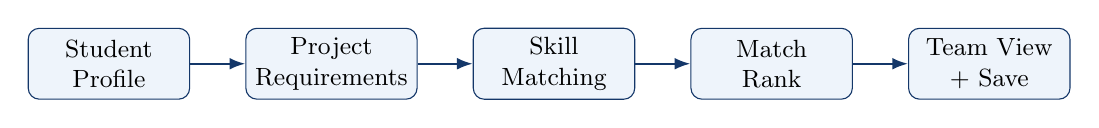
\begin{tikzpicture}[
node distance=7mm,
box/.style={rectangle,rounded corners,draw=GEUBlue,fill=GEULightBlue,
minimum width=2.05cm,minimum height=9mm,align=center,font=\small},
arrow/.style={-{Latex[length=2mm]},thick,draw=GEUBlue}
]
\node[box] (a) {Student\\Profile};
\node[box,right=of a] (b) {Project\\Requirements};
\node[box,right=of b] (c) {Skill\\Matching};
\node[box,right=of c] (d) {Match\\Rank};
\node[box,right=of d] (e) {Team View\\+ Save};
\draw[arrow] (a)--(b); \draw[arrow] (b)--(c); \draw[arrow] (c)--(d); \draw[arrow] (d)--(e);
\end{tikzpicture}
\end{center}
\vspace{4mm}
\begin{columns}[T,totalwidth=\textwidth]
\column{.48\textwidth}
\textbf{\color{GEUBlue}Major Components}
\begin{itemize}\setlength{\itemsep}{2pt}
\item Profile Manager + Requirement Manager
\item Matching Engine + Ranking
\item Team Manager + local storage
\end{itemize}
\column{.48\textwidth}
\textbf{\color{GEUBlue}Data / Control Flow}
\begin{itemize}\setlength{\itemsep}{2pt}
\item Profile \textrightarrow skills \textrightarrow candidate retrieval
\item Candidate set \textrightarrow score \textrightarrow ranking
\item Team selection \textrightarrow coverage check \textrightarrow save
\end{itemize}
\end{columns}
\end{frame}

% 8
\begin{frame}{Technology Stack \& Methodology}
\begin{columns}[T,totalwidth=\textwidth]
\column{.48\textwidth}
\begin{block}{Technology Stack}
\begin{itemize}\setlength{\itemsep}{2pt}
\item Programming: C++
\item UI Framework: Qt
\item Storage: Local structured files
\item IDE: VS Code / Qt Creator
\item Version Control: Git / GitHub
\end{itemize}
\end{block}
\column{.48\textwidth}
\begin{block}{Development Methodology}
\begin{enumerate}\setlength{\itemsep}{2pt}
\item Requirement Analysis
\item System Design
\item Implementation
\item Testing
\item Evaluation
\end{enumerate}
\end{block}
\end{columns}
\vfill
\smallnote{Qt was selected for the desktop UI after mentor discussion. It provides the interface tools needed for the C++ application.}
\end{frame}

% 9
\begin{frame}{Initial Progress \& Team Contribution}
\footnotesize
\begin{columns}[T,totalwidth=\textwidth]
\column{.43\textwidth}
\textbf{\color{GEUBlue}Progress Achieved}
\begin{itemize}\setlength{\itemsep}{2pt}
\item Discussed multiple project ideas with the mentor.
\item TeamForge was approved on 31 Aug 2026; problem, users and features were fixed.
\item User flow and architecture were drafted.
\item C++ with Qt was selected; initial matching was discussed.
\end{itemize}
\column{.54\textwidth}
\textbf{\color{GEUBlue}Individual Contribution}
\vspace{2mm}
\tiny
\begin{tabularx}{\textwidth}{@{}p{1.5cm}p{1.9cm}X@{}}
\toprule
Member & Role & Contribution\\
\midrule
Mukul Fartiyal & Team / Integration Lead & Requirements, architecture and coordination.\\
Anubhav Bisht & UI / Testing / Documentation Lead & Qt UI planning, testing plan and documentation.\\
Siddhant Singh & C++ / OOP Lead & C++ class design and application structure.\\
Mehul & DSA Lead & Matching, searching, hashing and ranking.\\
\bottomrule
\end{tabularx}
\end{columns}
\end{frame}

% 10
\begin{frame}[t]{Roadmap, Expected Outcomes \& References}
\small
\begin{columns}[T,totalwidth=\textwidth]
\column{.47\textwidth}
\textbf{\color{GEUBlue}Roadmap}
\begin{enumerate}\setlength{\itemsep}{1pt}
\item Phase-I: Topic approval, requirements and design.
\item Phase-II: Application and matching development.
\item Phase-III: Testing, refinement and final demonstration.
\end{enumerate}
\vspace{0.5mm}
\textbf{\color{GEUBlue}Expected Outcomes}
\begin{itemize}\setlength{\itemsep}{0pt}
\item C++ / Qt desktop prototype.
\item Ranked teammate recommendations.
\item Coverage + local storage.
\end{itemize}
\column{.47\textwidth}
\textbf{\color{GEUBlue}References}
\begin{enumerate}\setlength{\itemsep}{1pt}
\item Qt Documentation, Qt Widgets and Layouts.
\item cppreference.com, C++ Standard Library Reference.
\item Reema Thareja, \textit{Data Structures Using C}, Oxford University Press.
\item E. Balagurusamy, \textit{Object Oriented Programming with C++}.
\end{enumerate}
\vspace{0mm}
\begin{center}
\colorbox{GEUBlue}{\parbox{.76\textwidth}{\centering\color{white}\textbf{Thank You}\\Questions \& Suggestions}}
\end{center}
\end{columns}
\end{frame}

\end{document}
